% -- Implementation ---------------------------------------

\section{Implementation}

Our extracted kernel can be found in \ref{app:satd}. In order to make the extracted kernel qualified for compilation and execution, a few things have to be altered. First, the new file has to be recognized by the makefile in the rovex-examples directory. By executing make byte-<kernel> two files are created:
\begin{itemize}
	\item bytecode, containing all the intstructions to be executed by the $\rho$-VEX
	\item bytedata, containing the pixels of the input stream
\end{itemize}

Second, some type definitions have to be made. Originally, pixel\_satd\_8x4 resides in the pixel.c file of the x264 application. When extracting this kernel, all prior knowledge is lost and has to be defined again. Then, in order to make the kernel compile and run on the $\rho$-VEX, the development board has to be reset and started. Bytecode has to be written to the instruction memory (rvex-imemory) and bytedata to the data memory (rvex-dmemory). Finally, the calculated result should be returned to the host. Figure X shows the $\rho$-VEX memory layout for our kernel.

\subsection{Adjusting the makefile}

In order to make the makefile recognize the extracted kernel, the file can simply be added to the EXECUTABLES. Other files are already in the makefile (e.g. adpcm), but these can be removed since we will not need them for our application. An important issue is the difference between logical memory and physical memory. While the first address of a logical memory is obviously zero, the physical memory can have the first part of the register being occupied by the operating system creating a so-called stride. For the $\rho$-VEX, this stride appeared to be 120. Thus, when writing for example the result of the kernel to the logical address '0', it actually should be written to the physical address '120' of the data memory. This can be done using \_\_DATA\_START to indicate the start address.

Despite the fact that this is a rather simplistic operation, it took us some struggling to have this action confirmed as correct. For example, we were told to remove the AUTOINLINE flag which resulted in a lot of wrong hexdumps. Also, half way the lab a fix has been made to eliminate the issue of the stride. All references to \_\_DATA\_START had to be removed again, which felt like we had wasted lots of time. Unfortunately, we still had major problems getting the application to run correctly. As it turned out, the fix had only affected the 'home' directory. In order to avoid conflicting files, we had created a separate folder named 'lab2' from where we executed the application. Due to this, the fix did not reach our code and thus did not eliminate the stride issue.

\subsection{Type Definition}

As stated earlier, an extracted kernel is unable to obtain information from previous code. Consequently, all parameters have to be pre-defined. Table \ref{typedef} shows all required type definitions.

% -- Type Definitions ---------------------------------------
\begin{table}[htb]%
\begin{tabular}{lll}
	\bf{Parameter} 	& \bf{Type definition} 	& \bf{Motivation}\\ \cline{1-3}
	intptr\_t				&	unsigned int					& This parameter represents the stride, which cannot be $<$0\\
	pixel						& unsigned char					&	Pixels are made out of bytes, which have 8 bits (like a char)\\
	sum\_t					&	short int							& Same type definition as in the source code (16 bits)\\
	sum2\_t					& long int							& Same type definition as in the source code (32 bits)\\
	BIT\_DEPTH			& defined as 8					& Also in the source code, plus the kernel handles pixels (bytes)\\
	BIT\_PER\_SUM		&	(8 * sizeof(sum\_t))	& Also predefined as in the source code, being 8 as well\\
\end{tabular}
\caption{Type definitions in the extracted kernel file.}
\label{typedef}
\end{table}

\subsection{Communication between the MicroBlaze and the $\rho$-VEX}

In order to delegate the satd\_8x4 kernel from the MicroBlaze to the $\rho$-VEX, both the environments need to communicate with each other. When executing the x264 application, the MicroBlaze has to load the instructions of the extracted kernel into the instruction memory of the $\rho$-VEX and the data (for which the SATD has to be evaluated) into the data memory. This is when the x264 becomes involved. The pixel\_satd\_8x4 kernel, which is residing in the pixel.c file of the application, needs to be overwritten. Instead of calculating the SATD, it should send the instructions and input to the $\rho$-VEX. The commands \ref{eq:imem} and \ref{eq:dmem} are therefore added to the pixel.c file of the x264 application.

\begin{figure}
	\centering
	\begin{subfigure} [h] {0.3\textwidth}
		\centering
		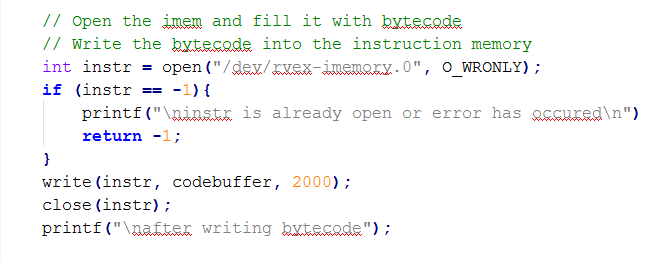
\includegraphics[width=150px]{Pictures/imem}
		\caption{Bytecode}
		\label{fig:imem}
	\end{subfigure}
	\quad
	\begin{subfigure} [h] {0.3\textwidth}
		\centering
		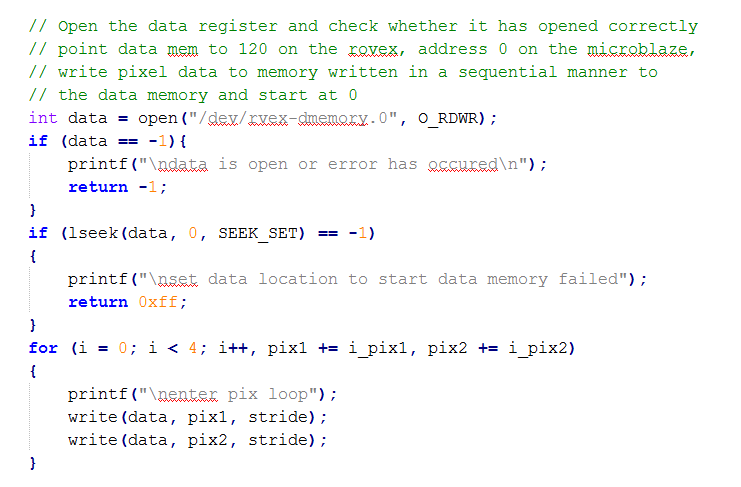
\includegraphics[width=150px]{Pictures/dmem}
		\caption{Bytedata}
		\label{fig:schottky2}
	\end{subfigure}
	\quad
\caption{Commands for loading the bytecode and bytedata into the $\rho$-VEX}%
\label{}%
\end{figure}